% Ch4.tex

\chapter[Frog call classification based on enhanced features]{Frog call classification based on enhanced features and machine learning algorithms}
\label{cha:cha4EnhancedFeature}



\section{Introduction}
\label{S:1}

This chapter presents an enhanced feature representation for the frog call classification using various machine learning algorithms. In the literature, various feature representations have been developed for frog call classification. However, most features used in the prior work are based on either temporal features, perceptual features, or cepstral features. Is it that a combination of three types of features can discriminate a wider variety of species that may share similar characteristics in either temporal, perceptual or cepstral information but not all?

This chapter aims to compare various feature representations with different machine learning techniques. Based on the classification performance, suggested features can then be transplanted to study low-SNR recordings. This chapter directly addresses sub-research question 1(a): Various acoustic features have been developed to classify frog calls in high SNR recordings; which of those features can be transplanted from high SNR recordings to low SNR recordings?

The performance of the proposed method is evaluated based on twenty-four frog species, which are geographically well distributed through Queensland, Australia. Five feature representations are compared via five machine learning algorithms. Classification results demonstrate a combination of temporal, spectral and cepstral features can achieve the best performance. Compared with temporal and spectral features, cepstral features can achieve a robust classification accuracy, but sensitive to the background noise. Therefore, in the next chapter, we aim to develop a robust cepstral features that are not sensitive to the background noise.




\section{Journal paper - Acoustic classification of Australian frogs based on enhanced features and machine learning algorithms}


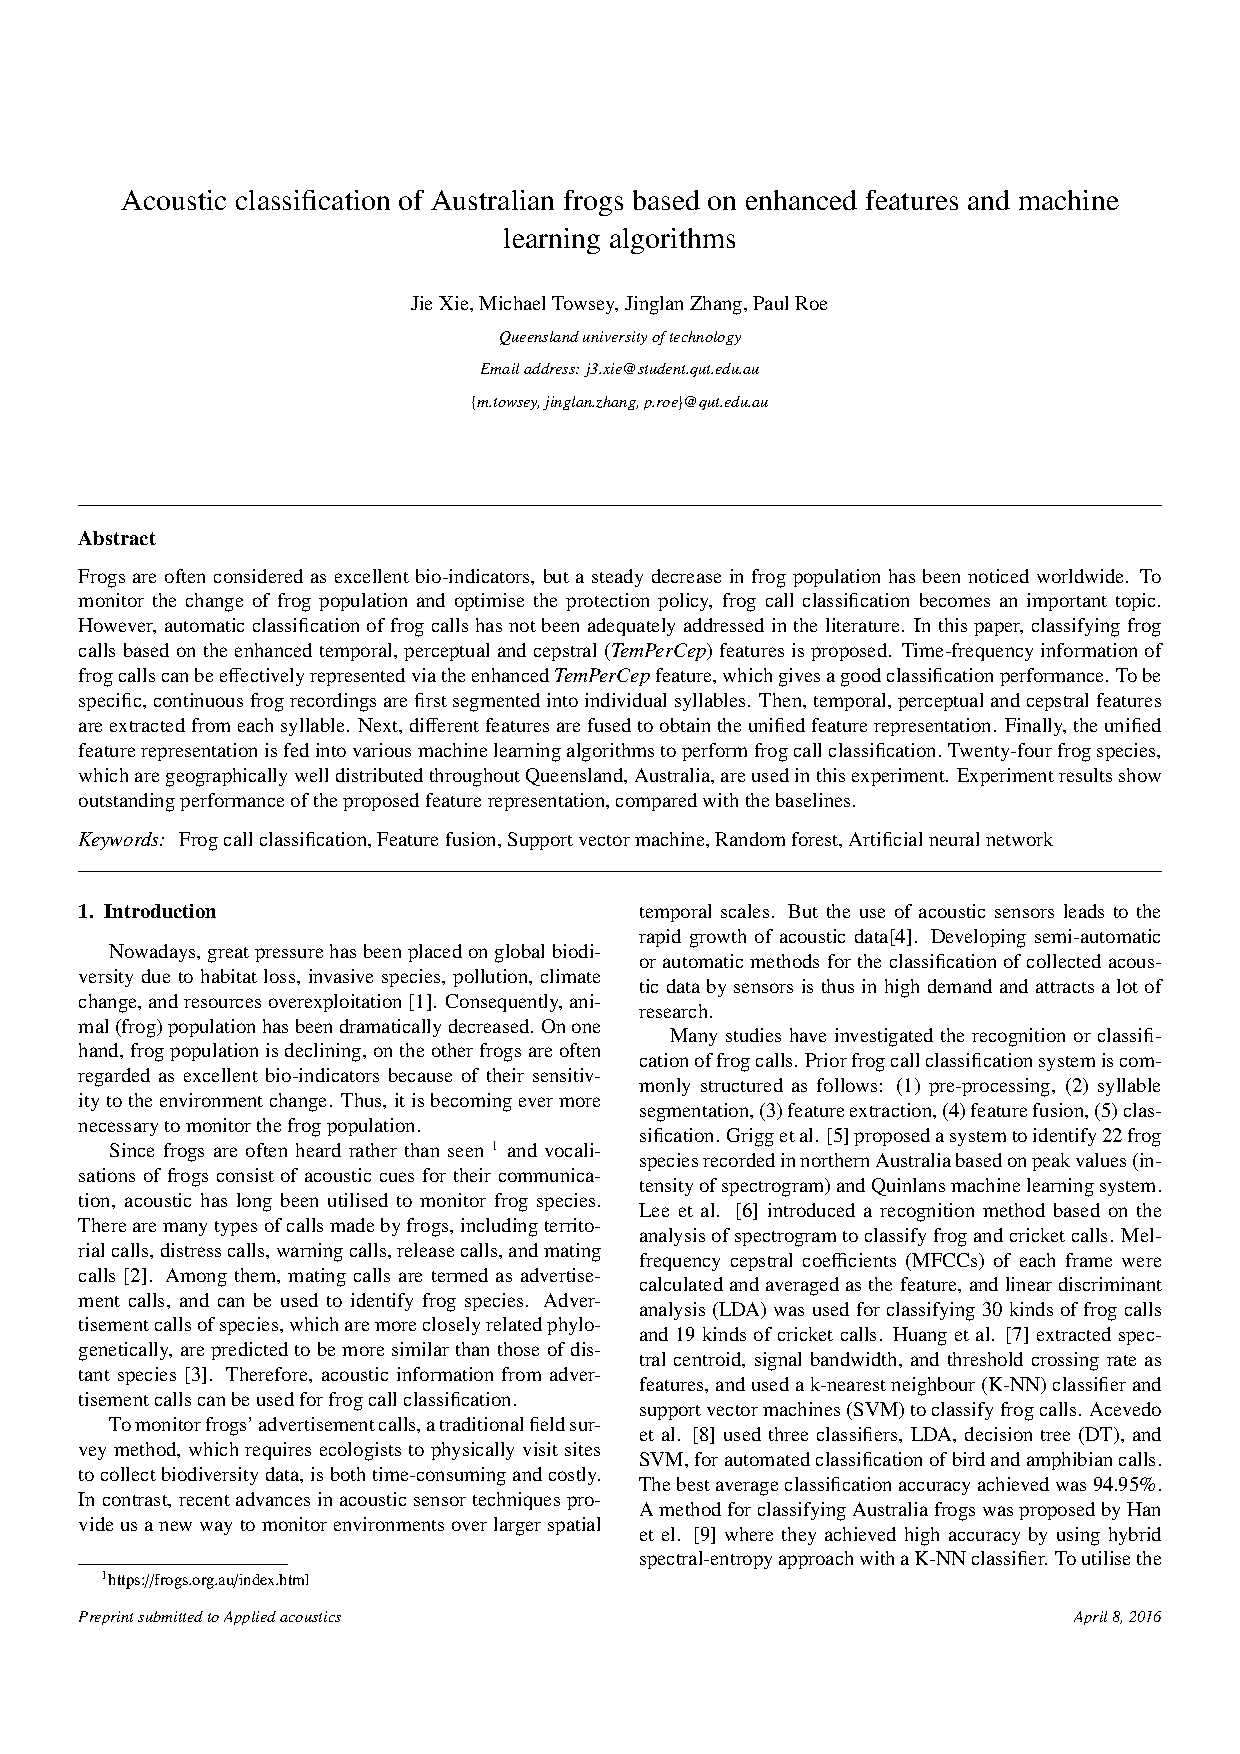
\includepdf[pages=-, pagecommand={},width=1.2\textwidth]{Ch4_paper.pdf}
